\section{Porównywanie wydajności zapytań}
W rozdziale przedstawiono działanie polecenia EXPLAIN, które pozwala uzyskać informacje o planie wykonania zapytania i jest podstawową metodą określenia sposobu wykonywania zapytań przez serwer MySQL. Analiza wyników polecenia EXPLAIN jest zdecydowanie bardziej miarodajna od mierzenia czasów zapytań. Na czas wykonania zapytania mają wpływ zewnętrzne czynniki, które mogą wprowadzić w błąd, podczas badania wydajności zapytania jedynie na podstawie czasu jego wykonania. 

Pierwszym z nich jest bufor zapytań. Przeprowadzając testy zapytania przy włączonym buforze zapytań, może zdarzyć się, że rezultat zapytania zostanie zwrócony błyskawicznie z bufora zapytań. Doprowadzi to do sytuacji, kiedy nawet najbardziej niewydajne zapytania będą zwracane nieproporcjonalnie szybko. Problem ze zwracaniem wyników z bufora zapytań można rozwiązać poprzez wyłączenie bufora zapytań lub dodanie modyfikatora SQL\textunderscore NO\textunderscore CACHE do zapytań. 
Drugim czynnikiem zaburzającym mierzenie czasów wykonania zapytań jest bufor MySQL. MySQL stara się przechowywać w pamięci często używane dane, przykładowo indeksy lub nawet często pobierane dane. Jeżeli wykonujemy zapytanie dla tabeli, której indeks nie znajduje się w pamięci, serwer pobiera indeks z dysku, a taka operacja wymaga dodatkowego nakładu na pobranie danych do pamięci, co skutkuje wydłużeniem czasu wykonania zapytania. Wykonując kolejne zapytanie, może okazać się, że pomimo pogorszenia jego wydajności, zostanie ono wykonane w krótszym czasie (ze względu na różnicę w czasie dostępu do pamięci i dysku twardego). Mierząc jedynie czasy wykonania obu zapytań, można dojść do fałszywego wniosku, że drugie zapytanie jest wydajniejsze, nawet jeżeli w rzeczywistości nasze działanie doprowadziło do pogorszenia wydajności. Problem ten może zostać rozwiązany poprzez obliczenie średniego czasu i na jego podstawie porównywanie wyników. Takie rozwiązanie jednak wciąż nie gwarantuje deterministycznego charakteru porównania.

Dodatkowo baza danych rzadko kiedy jest całkowicie odcięty od świata. Z reguły testowanie wydajności będzie odbywać się dla tabeli, które są w jednocześnie modyfikowane przez inne połaczenia. Przykładowo, jeżeli testowane jest zapytanie na tabeli, na której w tym samym czasie wykonywane są operacje zapisu; porównanie czasów wykonania zapytań nie musi być miarodajne.

Na czasy wykonywania zapytań wpływać może również aktualne obciążenie serwera. Wyniki czasów wykonania zapytań będą wyraźnie zależeć od aktualnego poziomu wykorzystania zasobów serwera.

Po przeanalizowaniu powyższych ograniczeń metody analizy wydajności zapytań można stwierdzić, że operowanie tylko na takiej metodzie jest obarczone wyraźnym błędem i nie powinno być jedynym sposobem porównywania wydajności.
\subsection{Polecenie EXPLAIN}
Polecenie EXPLAIN będzie jedną z głównych metod porównywania wydajności zapytań stosowaną w tej pracy, dlatego w tym podrozdziale przedstawiono podstawowy jego stosowania. 

Język SQL jest językiem deklaratywnym. Decyzję o sposobie przechowywania i pobrania danych pozostawia się systemowi zarządzania bazą danych. Funkcja EXPLAIN służy do określenia sposobu, w jaki baza danych wykona zapytanie.

Aby użyć polecenia EXPLAIN, należy poprzedzić słowa kluczowe takie jak SELECT,INSERT,UPDATE,DELETE poleceniem EXPLAIN. Spowoduje to, że zamiast wykonania zapytania, baza danych zwróci informacje o planie jego wykonania. Rezultat polecenia EXPLAIN zawiera po jednym rekordzie dla każdej tabeli użytej w zapytaniu, chociaż czasami może zawierać również tabele stworzone przez serwer w pamięci. Kolejność wierszy w wyniku zapytania odpowiada kolejności, w jakiej MySQL będzie je wykonywał. Pierwszym zapytaniem wykonanym przez MySQL będzie zapytanie z ostatniego wiersza.

\subsection{Wyniki polecenia EXPLAIN}
W celu zademonstrowania wyników polecenia EXPLAIN na rzeczywistych przykładach, wykonano polecenie EXPLAIN dla kilku zapytań na bazie StackOverflow .Zapytania są ponumerowane względem kolejności ich występowania w rozdziale.
\begin{spverbatim}
	SELECT u.DisplayName, c.CreationDate, c.`Text` FROM  Comments c LEFT JOIN Users u ON c.UserId = u.Id WHERE c.PostId = 875;
\end{spverbatim}
\begin{figure}[H]
	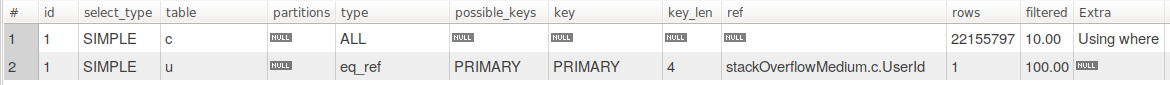
\includegraphics[scale =0.4]{explain7.png} 
	\caption{Przykład 1}
\end{figure}
\begin{spverbatim}
	SELECT p.Body FROM Posts p WHERE p.Id = 875 UNION
	SELECT c.`Text` FROM Comments c WHERE c.PostID = 875;
\end{spverbatim}
\begin{figure}[H]
	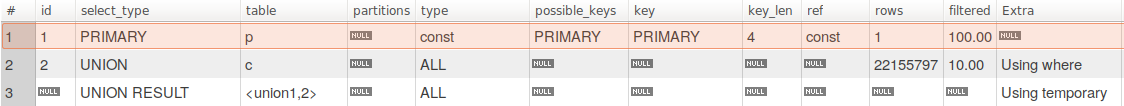
\includegraphics[scale =0.4]{explain8.png} 
	\caption{Przykład 2}
\end{figure}
\begin{spverbatim}
	SELECT * FROM Comments WHERE UserId = (SELECT id FROM Users WHERE DisplayName = 'Jarrod Dixon');
\end{spverbatim}
\begin{figure}[H]
	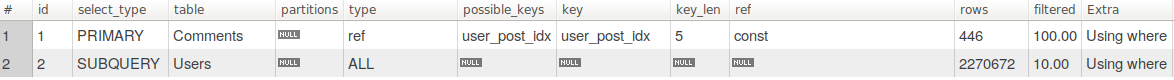
\includegraphics[scale =0.4]{explain9.png} 
	\caption{Przykład 3}
\end{figure}
\begin{spverbatim}
	SELECT * FROM Comments WHERE UserID in (SELECT UserId FROM Posts GROUP BY UserId HAVING COUNT(*) > 10);
\end{spverbatim}
\begin{figure}[H]
	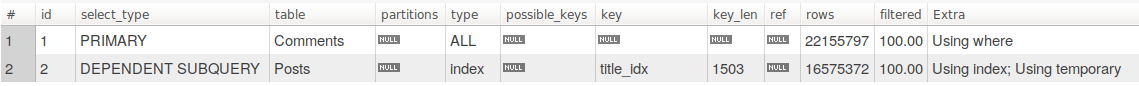
\includegraphics[scale =0.4]{explain9a.png} 
	\caption{Przykład 4}
\end{figure}
\begin{spverbatim}
	SELECT * FROM Comments WHERE UserID in (SELECT UserId FROM Posts GROUP BY UserId HAVING COUNT(*) > 10);
\end{spverbatim}
\begin{figure}[H]
	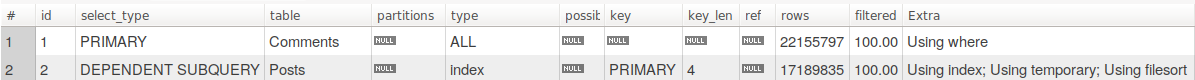
\includegraphics[scale =0.4]{explain10.png} 
	\caption{Przykład 5}
\end{figure}
\begin{spverbatim}
	SELECT * FROM Posts  WHERE OwnerUserId IN (SELECT id FROM Users WHERE Reputation>1000 UNION SELECT UserId FROM Comments WHERE Score >10)
\end{spverbatim}
\begin{figure}[H]
	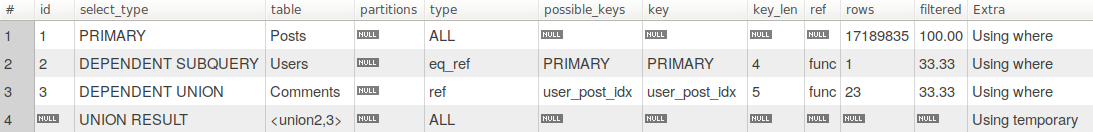
\includegraphics[scale =0.4]{explain11.png} 
	\caption{Przykład 6}
\end{figure}
\begin{spverbatim}
	SELECT * FROM Comments WHERE UserId = (SELECT @var1 FROM Users WHERE DisplayName = 'Jarrod Dixon');
\end{spverbatim}
\begin{figure}[H]
	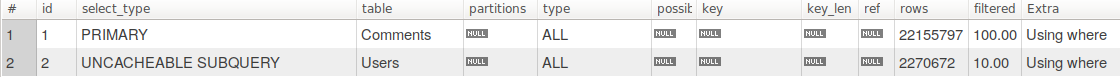
\includegraphics[scale =0.4]{explain12.png} 
	\caption{Przykład 7}
\end{figure}
\begin{spverbatim}
SELECT * FROM Comments LIMIT 10;
\end{spverbatim}
\begin{figure}[H]
	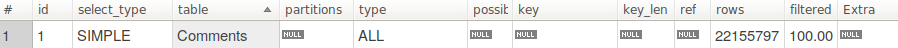
\includegraphics[scale =0.4]{explain13.png} 
	\caption{Przykład 8}
\end{figure}
\begin{spverbatim}
	SELECT * FROM Users WHERE Id BETWEEN 1 AND 100 AND 
	id NOT IN (SELECT OwnerUserId FROM Posts WHERE Score >100);
\end{spverbatim}
\begin{figure}[H]
	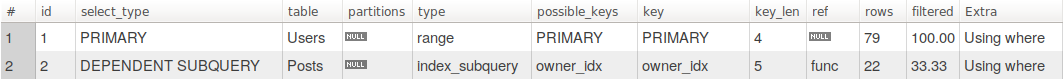
\includegraphics[scale =0.4]{explain24.png} 
	\caption{Przykład 9}
\end{figure}
\begin{spverbatim}
	SELECT * FROM Comments WHERE UserId = 20500 OR id = 20500;
\end{spverbatim}
\begin{figure}[H]
	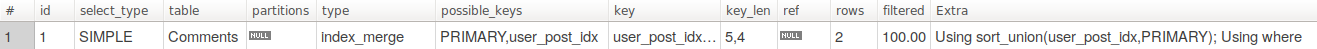
\includegraphics[scale =0.3]{explain25.png} 
	\caption{Przykład 10}
\end{figure}

\subsubsection{Kolumna \#}
Wartości w kolumnie \# określają kolejność, w jakiej MySQL będzie odczytywał tabele. Jako pierwsza odczytywana jest tabela z najmniejszą wartością.

\subsubsection{Kolumna ID}\leavevmode\\
Kolumna id zawiera numer zapytania, którego dotyczy. W przypadku zapytań z podzapytaniami, podzapytania w dyrektywie FROM oraz zapytań ze słowem kluczowym JOIN, numerowane są najczęściej względem ich występowania w zapytaniu. Kolumna ID może przyjąć również wartość NULL, w przypadku polecenia UNION (przykład 2).

\subsubsection{Kolumna select\textunderscore type}\leavevmode\\
Kolumna select\textunderscore informuje o rodzaju wykonywanego zapytania SELECT. 
Poniżej przedstawiono wartości, które mogą zostać zwrócone dla tej kolumny.
\begin{itemize}
	\item \textbf{SIMPLE} Wartość SIMPLE oznacza, że zapytanie nie zawiera podzapytań, oraz nie używa złączeń (klauzula UNION).
	\item \textbf{PRIMARY} Jeżeli zapytanie zawiera podzapytania lub wykorzystuje złaczenie, to rekord dla kolumny select\textunderscore type przyjmie wartość PRIMARY (przykład 2).
	\item \textbf{SUBQUERY} Jeżeli rekord dotyczy podzapytania oznaczonego jako PRIMARY, to zostanie oznaczony jako SUBQUERY (przykład 3)
	\item \textbf{UNION} Jako UNION zostaną oznaczone zapytania, które są drugim i kolejnym zapytaniem operacji złączenia tabel. Pierwsze zapytanie zostanie oznaczone tak samo, jakby było wykonywane jako zwykłe zapytanie SELECT (przykład 2).
	\item \textbf{\textbf{DERIVED}} Oznacza, że zapytanie jest umieszczone jako podzapytanie w klauzuli FROM, jest wykonywane rekurencyjnie i wyniki są umieszczane w tabeli tymczasowej.
	\item \textbf{UNION RESULT} Oznacza wiersz, w którym polecenie SELECT zostało użyte do pobrania wyników z tabeli tymczasowej użytej przy poleceniu UNION (przykład 2).
	\item \textbf{DEPENDENT SUBQUERY} Jeśli polecenie SELECT zależy od danych znajdujących się w podzapytaniu (przykład 5).
	\item \textbf{DEPENDENT UNION} Jeśli polecenie SELECT zależy od danych znajdujących się w tabeli tymczasowej bedącej wynikiem złączenia (przykład 6).
	\item \textbf{\textbf{MATERIALIZED}} Jeżeli wynik zwracany jest ze \textit{zmaterializowanego widoku (eng. materialized view)}. Widok zmaterializowany jest obiektem bazy danych zawierającym rezultat zapytania.
	\item \textbf{UNCACHABLE\textunderscore SUBQUERY}. Oznaczający, że zapytanie nie może być buforowane (przykład 7).
	\item \textbf{UNCACHABLE\textunderscore UNION}. Oznaczający, że wynik złączenia tabel nie może zostać buforowany.
\end{itemize}

\subsubsection{Kolumna table}\leavevmode\\
Kolumna \textit{table} w większości przypadków zawiera nazwę tabeli lub jej alias, do której odnosi się dany wiersz wyniku polecenia \textit{EXPLAIN}. Gdy zapytanie dotyczy tabel tymczasowych, możemy zobaczyć np. table: <union1,2> (przykład 2), co oznacza, że zapytanie dotyczy tabeli tymczasowej stworzonej na podstawie polecenia \textit{UNION} na tabelach z wierszy o id 1 oraz 2.
Odczytując kolejno wartości kolumny \textit{table} możemy dowiedzieć się, w jakiej kolejności optymalizator MySQL zdecydował się ułożyć zapytania. 

\subsubsection{Kolumna Type}\leavevmode\\
Kolumna \textit{Type} informuje o tym, w jaki sposób MySQL będzie przetwarzał wiersze w tabeli. Poniżej przedstawiono najważniejsze metody dostępu do danych, w kolejności od najgorszej do najlepszej.

\begin{itemize}
	\item \textbf{ALL} 
	
	\newline	Wartość \textit{ALL} informuje o tym, że serwer musi przeskanować całą tabelę w celu odnalezienia rekordów. Istnieją jednak wyjątki takie, jak w przykładzie 8, w którym polecenie \textit{EXPLAIN} pokazuje, że będzie wykonywany pełny skan tabeli, a w rzeczywistości dzięki użyciu polecenia \textit{LIMIT} zapytanie będzie wymagało jedynie 10 rekordów.
	\item \textbf{Index} 
	\newline MySQL skanuje wszystkie wiersze w tabeli, ale może wykonać to w porządku, w jakim jest przechowywane w indeksie, dzięki czemu unika sortowania. Największą wadą jest jednak nadal konieczność odczytu całej tabeli. Co więcej, dane z dysku pobierane są z adresów, których kolejność wynika z użytego indeksu. Adresy te nie muszą zajmować na dysku ciągłych obszarów, a to oznacza, że czas odczytu danych może znacznie wydłużyć się. Jeżeli w kolumnie \textit{extra} jest dodatkowo zawarta informacja ''Using Index'' oznacza to, ze MySQL wykorzystuje indeks pokrywający (opisany w dalszej części pracy) i nie wymaga odczytywania innych danych z dysku – do wykonania zapytania wystarczają dane umieszczone w indeksie.
	\item \textbf{Range} \newline
	Wartość \textit{range} oznacza ograniczone skanowanie zakresu. Takie skanowanie rozpoczyna się od pewnego miejsca indeksu, dzięki czemu nie musimy przechodzić przez cały indeks. Skanowanie indeksu powodują zapytania zawierające klauzulę \textit{BETWEEN} lub \textit{WHERE} z < lub >. Wady są takie same jak przy rodzaju \textit{index}
	\item \textbf{Index\textunderscore subquery} \newline Tego typu zapytanie zostało przedstawione w przykładzie 9, w którym podzapytanie korzysta z nieunikalnego indeksu, jest wykonane przed głównym zapytaniem i jego wartości są przekazane do niego jako stałe.
	\item\textbf{Unique\textunderscore subquery} \newline Analogicznie do \textit{index\textunderscore subquery}, ale tym razem z użyciem klucza głównego lub indeksu UNIQUE NOT NULL.
	\item \textbf{Index\textunderscore merge}
\newline Czasami jeden indeks nie wystarczy do efektywnego wykonania zapytania. W  przykładzie 10 na tabeli \textit{Comments} założono dwa różne indeksy, obejmujące obie kolumny występujące w zapytaniu. Użycie tylko jednego indeksu poprawi  efektywność zapytania w ograniczonym stopniu, ponieważ serwer MySQL nadal musi przeprowadzić pełny skan tabeli. Dlatego od wersji 5.0 optymalizator może zdecydować się na złączenie kilku indeksów, dla efektywniejszego wykonania zapytania. Decyzja o tym, czy łączyć indeksy często zapada na podstawie rozmiaru tabeli. Przy tabelach niewielkich rozmiarów operacja złączenia może być kosztowniejsza niż pełny skan tabeli, ale przy dużych tabelach, przykładowo takich jak \textit{Comments} złączenie znacząco przyśpiesza wykonania zapytania. 
\item \textbf{Fulltext} \newline Wartość \textit{fulltext} oznacza, że wykorzystane zostało wyszukiwanie pełnotekstowe, opisane w dalszej części pracy.
\item \textbf{Ref}
\newline Jest to wyszukiwanie, w którym MySQL musi przeszukać jedynie indeks w celu znalezienia rekordu opowiadającego pojedynczej wartości.
Przykładem takiego zapytania jest wyszukiwanie numerów postów danego użytkownika w tabeli \textit{Comments} zawierającej indeks typu \textit{BTREE} na kolumnach \textit{UserId} oraz \textit{PostId}.

\begin{spverbatim}
	SELECT PostId FROM Comments WHERE UserId = 10;
\end{spverbatim}
Dodatkowo odmianą dostępu \textit{ref} jest \textit{ref\textunderscore or\textunderscore null}, który oznacza, że wymagany jest dodatkowy dostęp w celu sprawdzenia wartości NULL.

\item \textbf{Eq\textunderscore ref} \newline Jest to najlepsza możliwa forma złączenia. Oznacza, że z tabeli odczytywany jest tylko jeden wiersz dla każdej kombinacji wierszy z poprzednich tabel. Z tego rodzaju złączeniem mamy do czynienia, jeżeli wszystkie kolumny używane do złączenia są kluczem głównym lub indeksem ''NOT NULL UNIQUE''. Przykładem takiego zapytania jest złączenie wszystkich komentarzy z postami, bazując na kluczu głównym Id z tabeli Posts. 
\begin{spverbatim}
	SELECT * FROM Comments c JOIN Posts p ON c.PostId = p.id;
\end{spverbatim}

\item \textbf{Const} \newline 
Przeważnie występuje w przypadku użycia w klauzuli WHERE wartości z indeksu głównego. Wtedy wystarczy jednokrotne przeszukanie indeksu, a na znalezionym liściu indeksu dostępne są już wszystkie dane z wiersza tabeli. Przykładowo w bazie \textit{StackOverflow} może to być zapytanie, pobierające komentarz bazując na Id.
\begin{spverbatim}
	EXPLAIN SELECT * FROM Comments WHERE id = 93;
\end{spverbatim}


\item {\textbf{NULL}}
\newline

Oznacza, że serwer nie wymaga skanowania całej tabeli lub indeksu i może zwrócić wartość już podczas fazy optymalizacji. Przykładem takiego zapytania może być zwrócenie minimalnej wartości z indeksu tabeli.

\begin{spverbatim}
	SELECT MIN(UserId) FROM Comments;
	#Tabela Comments zawiera indeks BTREE na kolumnie UserID
\end{spverbatim}

\end{itemize}

\subsubsection{Kolumna Possible\textunderscore keys}
Komulna possible\textunderscore keys zawiera listę indeksów, które optymalizator brał pod uwagę podczas tworzenia planu wykonania zapytania. Lista tworzona jest na początku procesu optymalizacji zapytania.

\paragraph{Kolumna key}\leavevmode\\
Kolumna \textit{key} sygnalizuje, który indeks został wybrany do optymalizacji dostępu do tabeli.

\paragraph{Kolumna key\textunderscore len}\leavevmode\\
Wartość oznacza, jaki jest rozmiar bajtów użytego indeksu. W przypadku, kiedy zostanie wykorzystana jedynie część kolumn indeksu, wtedy wartość \textit{key\textunderscore len} będzie odpowiednio mniejsza. Istotny jest fakt, że rozmiar jest zawsze maksymalnym rozmiarem zindeksowanych kolumn, a nie rzeczywistą liczbą bajtów danych używanych do zapisu wiersza w tabeli.

\paragraph{Kolumna ref}\leavevmode\\
Kolumna pokazuje, które kolumny z innych tabel lub zmienne z innych tabel zostaną wykorzystane do wyszukania wartości w indeksie podanym w kolumnie \textit{key}. W przykładzie do przeszukania indeksu tabeli Posts wykorzystano kolumnę UserId z tabeli Comments (alias c). Wartość \textit{const} oznacza, że do przeszukania wartości została wykorzystana stała podana np. w klauzuli WHERE (Przykład 2). Kolumna może też przyjąć wartość \textit{func}, co oznacza, że wartość użyta do wyszukania jest wynikiem obliczenia pewnej funkcji (przykład 9).

\paragraph{Kolumna rows}\leavevmode\\
Kolumna wskazuje oszacowaną liczbę wierszy, które MySQL będzie musiał odczytać w celu znalezienia szukanych rekordów. Wartość może znacząco odbiegać od rzeczywistej liczby wierszy, które zostaną odczytane podczas wykonania zapytania. Jest to liczba przeszukiwanych rekordów na danym poziomie zagnieżdżenia pętli planu złączenia. Oznacza to, że nie jest to całkowita liczba rekordów, a jedynie liczba rekordów w jednej pętli złączenia danej tabeli. W przypadku złączenia sumaryczna liczba przeszukiwanych nie jest sumą wartości z wszystkich wierszy, a iloczynem wartości z wierszy biorących udział w złączeniu. W przykładzie 9 łączna suma wierszy, które muszą zostać przeszukane, nie wynosi 15748463.
\begin{spverbatim}
	SELECT * FROM Posts p JOIN PostTypes pt ON p.PostTypeId = pt.Id;
\end{spverbatim}
\begin{figure}[H]
	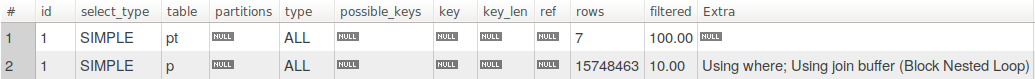
\includegraphics[scale =0.4]{explain14.png} 
	\caption{Przykład 9}
\end{figure}
Podczas szacowania wartości w kolumnie \textit{rows} optymalizator nie bierze pod uwagę klauzli \textit{LIMIT}.

\paragraph{Kolumna filtered}\leavevmode\\. Wskazuje na wartość oszacowaną przez optymalizator, która informuje, ile rekordów może zostać odfiltrowane za pomocą klauzuli WHERE. W przykładzie 4 optymalizator MySQL oszacował, że jedynie 10 procent użytkowników napisało w sumie więcej niż 10 komentarzy. Przed wersją 8.0, aby kolumna filtered była umieszczona w wynikach zapytania, należało wykorzystać polecenie EXPLAIN EXTENDED.

\paragraph{Kolumna extra}\leavevmode\\
Kolumna \textit{extra} zawiera informacje, których nie udało się zamieścić w pozostałych kolumnach. Poniżej przedstawiono kilka najważniejszych informacji, które mogą znaleźć się w tej kolumnie.

\begin{itemize}
	\item 'Using index' - MySQL użyje indeksu pokrywającego zamiast dostępu do tabeli.
	\item 'Using where' - oznacza, że MySQL przeprowadzi filtrowanie danych dopiero po wczytaniu danych z tabeli. Często jest to informacja, która może sugerować zmianę lub stworzenia nowego indeksu bądź całego zapytania.
	\item 'Using temporary' - do sortowania wyników używana jest tabela tymczasowa.
	\item 'Using filesort' - sortowanie nie może skorzystać z istniejących indeksów (nie ma odpowiedniego optymalnego indeksu), więc wiersze są sortowane za pomocą jednego z algorytmów sortowania.
	
\end{itemize}

\subsection{Podsumowanie}


Z opisu możliwości polecenia EXPLAIN zawartego w tym rozdziale wynika, że jego użycie niesie więcej informacji od mierzenia czasów wykonywanych operacji. Dzięki szczegółowym informacją na temat planu wykonania zapytania (termin opisany szerzej w rozdziale dotyczącym Optymalizatora MySQL) możliwe jest dokładniejsze zdefiniowanie przyczyn braku wydajności, jak i porównanie wydajności dwóch zapytań. Oczywiście nie można pominąć faktu, że dane przedstawione jako wynik analizy są zebrane na podstawie pewnych statystyk, które nie zawsze muszą być zbieżne z rzeczywistością. Z tego powodu mierzenie czasów może być skutecznym dopełnieniem analizy planu wykonania zapytania.